\section*{Introduction}\label{sec:introduction} % (fold)
This report explores the implementation and analysis of a 2D Lennard-Jones molecular dynamics simulation. In this project, we focus on two fundamental ensemble types in molecular mechanics: the microcanonical ensemble (NVE) and the canonical ensemble (NVT). \\
\\
The microcanonical ensemble (NVE) simulates an isolated system with a constant number of particles (N), volume (V), and total energy (E). The canonical ensemble (NVT), on the other hand, also has a constant number of particles (N) and volume (V), but in this case we keep the temperature (T) constant instead of the energy. This is done, in our case, by using a Berendsen thermostat.\\
\\
Both types of simulations employ the truncated Lennard-Jones potential, which models both the attractive and repulsive forces between particles.
\begin{equation}
	U_{\text {trunc }}(r)=\left\{\begin{array}{l}
		U(r)-U\left(r_c\right), \quad r \leq r_c \\
		0, \quad r>r_c
	\end{array} \quad, \text { with } \quad U(r)=4\left[\left(\frac{1}{r}\right)^{12}-\left(\frac{1}{r}\right)^6\right]\right.
\end{equation}
This potential is a fundamental model in computational physics and is most often used to accurately represents the behavior of noble gases. Furthermore the velocity-Verlet integration scheme is used to solve the equations of motion with the promise of having good computational efficiency and numerical stability.\\
\\
To improve performance, a cell lists based approach for finding neighboring particles, with the goal of significantly reducing the computational complexity from $O(N^2)$ to $O(N)$. In order to enhance our understand of the system, several key properties of the sytem were analyzed. This includes energy conservation, temperature equilibration, and the radial distribution, providing key insights into the structural organization of particles. \\
\\
By examining different temperatures and particle counts this project explores how system size and thermal energy affect particle dynamics and structural properties in both NVE and NVT ensembles.\\
\\
This project was implement using Python, for further information regarding the implementation, consult the README provided in projects root folder.

% section Introduction (end)
\section{Energy-Conserving Dynamics: The NVE Ensemble}\label{sec:energy_conserving_dynamics_the_nve_ensemble} % (fold)
% The microcanonical ensemble (NVE) represents an isolated system with fixed number of particles (N), volume (V), and total energy (E). In an ideal NVE simulation, the total energy should remain constant, providing a critical validation metric for our implementation. 
\begin{figure}[H]
	\centering
	\begin{subfigure}{0.5\textwidth}
		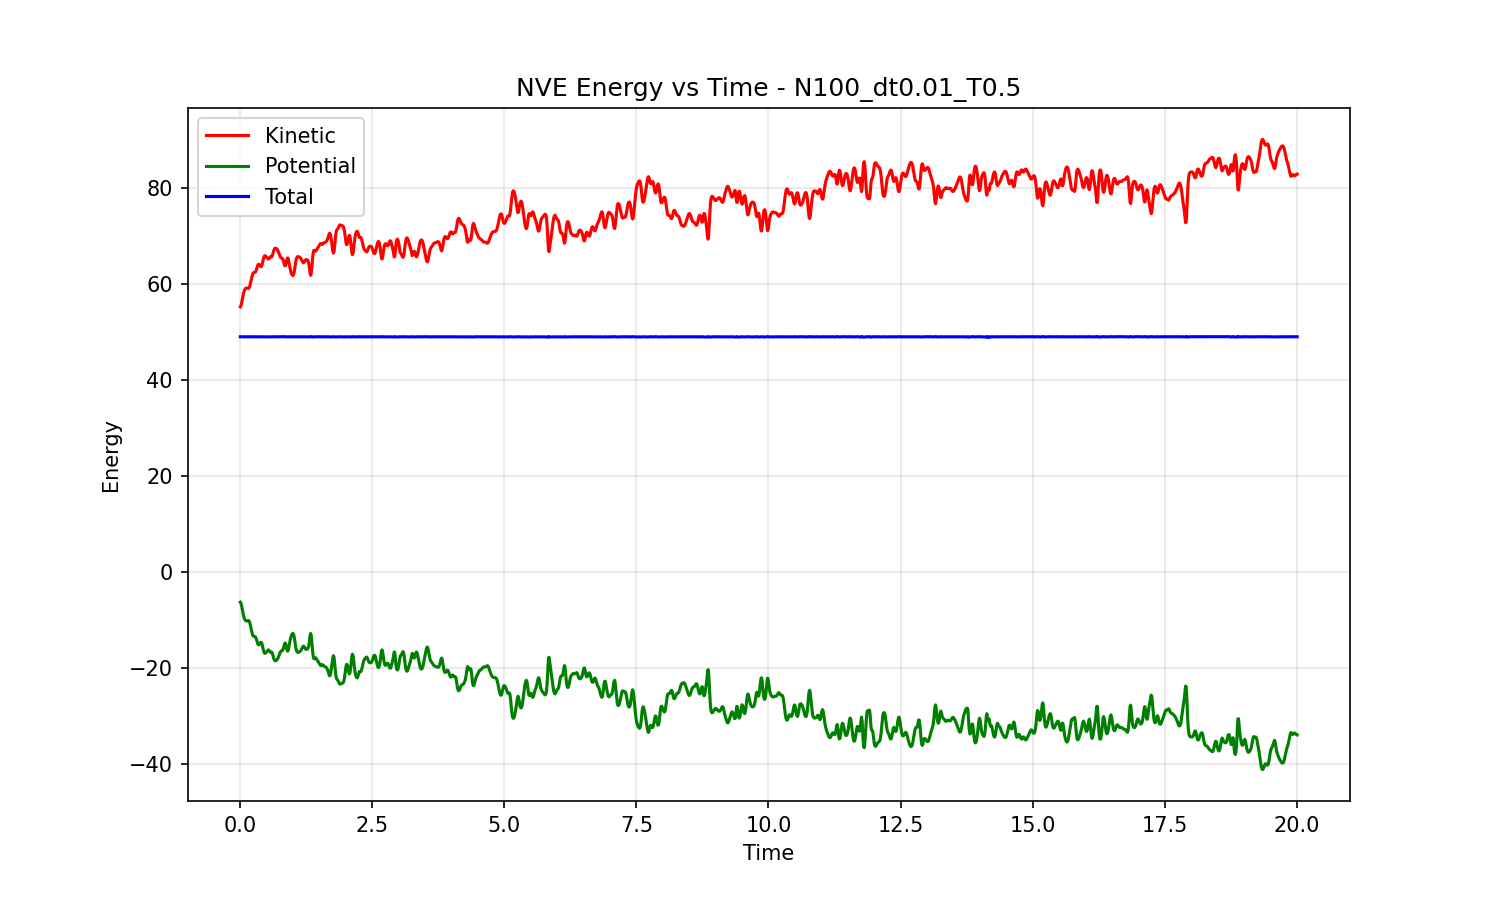
\includegraphics[width=\textwidth]{media/energy_N100_dt0.01_T0.5.png}
		\caption{N=100 particles with dt=0.01 and T=0.5}
		\label{sfig:energy_N100}
	\end{subfigure}%
	~
	\begin{subfigure}{0.5\textwidth}
		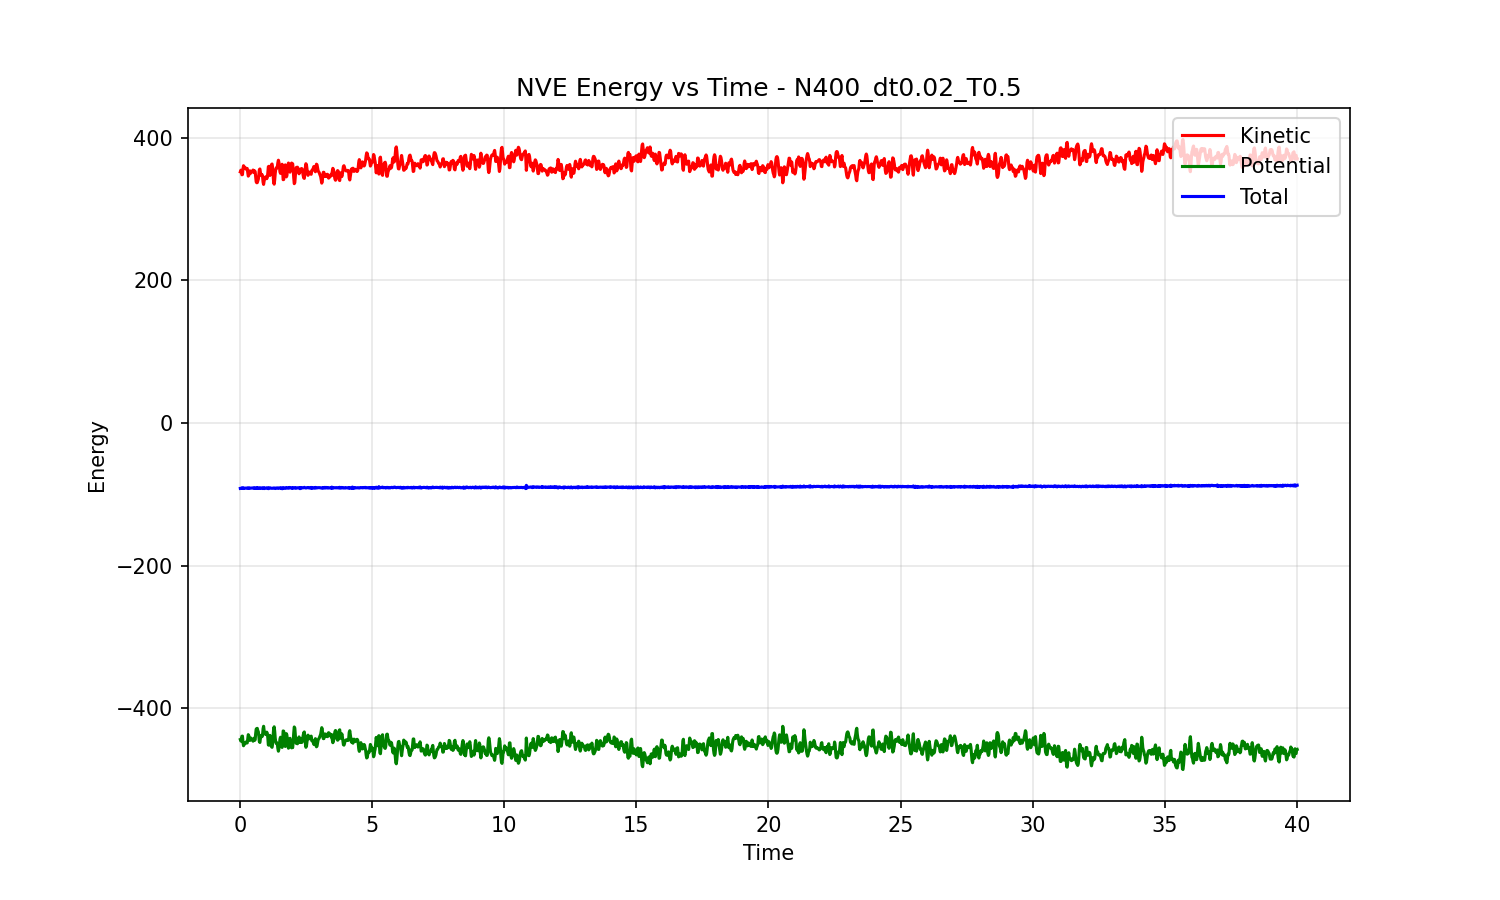
\includegraphics[width=\textwidth]{media/energy_N400_dt0.02_T0.5.png}
		\caption{N=400 particles with dt=0.02 and T=0.5}
		\label{sfig:energy_N400_dt002}
	\end{subfigure}%
	\\
	\begin{subfigure}{0.5\textwidth}
		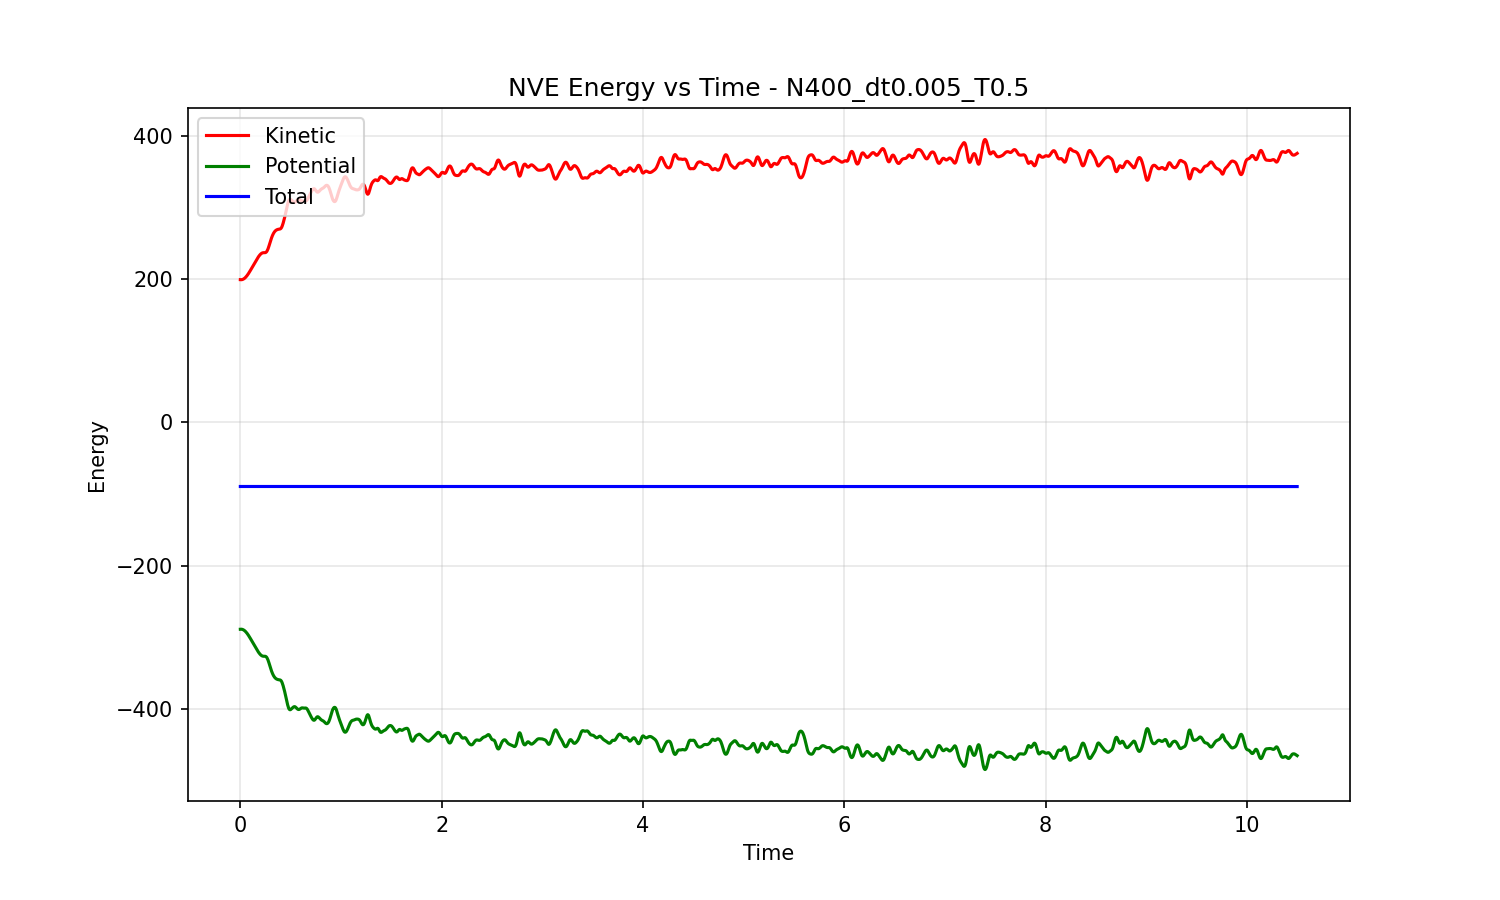
\includegraphics[width=\textwidth]{media/energy_N400_dt0.005_T0.5.png}
		\caption{N=400 particles with dt=0.005 and T=0.5}
		\label{sfig:energy_N400_dt0005}
	\end{subfigure}%
	~
	\begin{subfigure}{0.5\textwidth}
		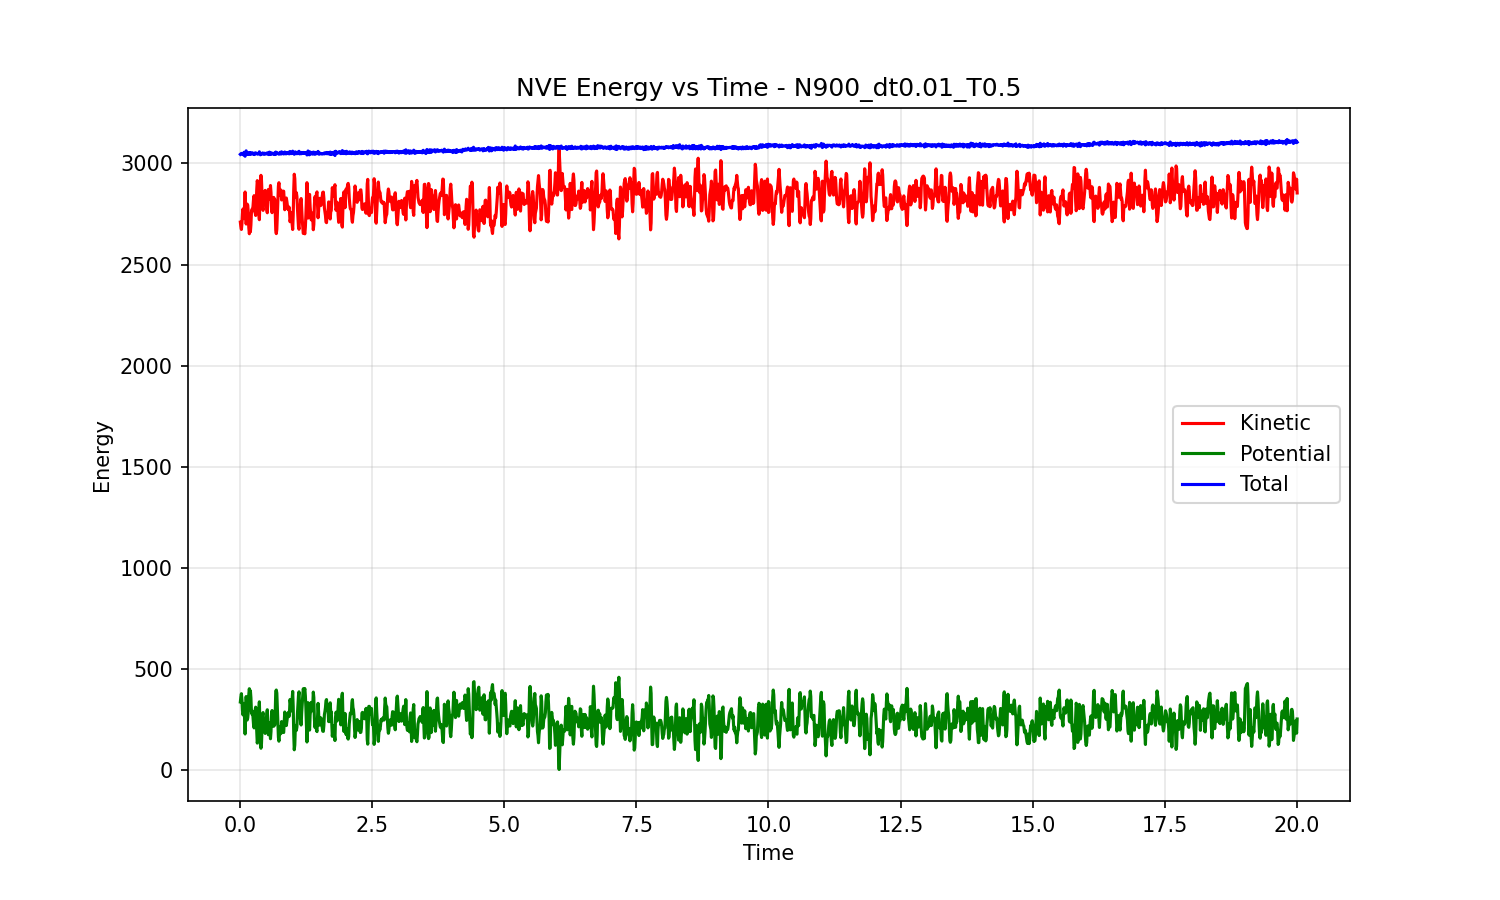
\includegraphics[width=\textwidth]{media/energy_N900_dt0.01_T0.5.png}
		\caption{N=900 particles with dt=0.01 and T=0.5}
		\label{sfig:energy_N900}
	\end{subfigure}%
	\caption{\textbf{Energy Conservation in NVE Ensemble} 
    Analysis of total, kinetic, and potential energies over time for different system configurations.}
	\label{fig:energy_conservation}
\end{figure}
\begin{figure}[H]
	\centering
	\begin{subfigure}{0.5\textwidth}
		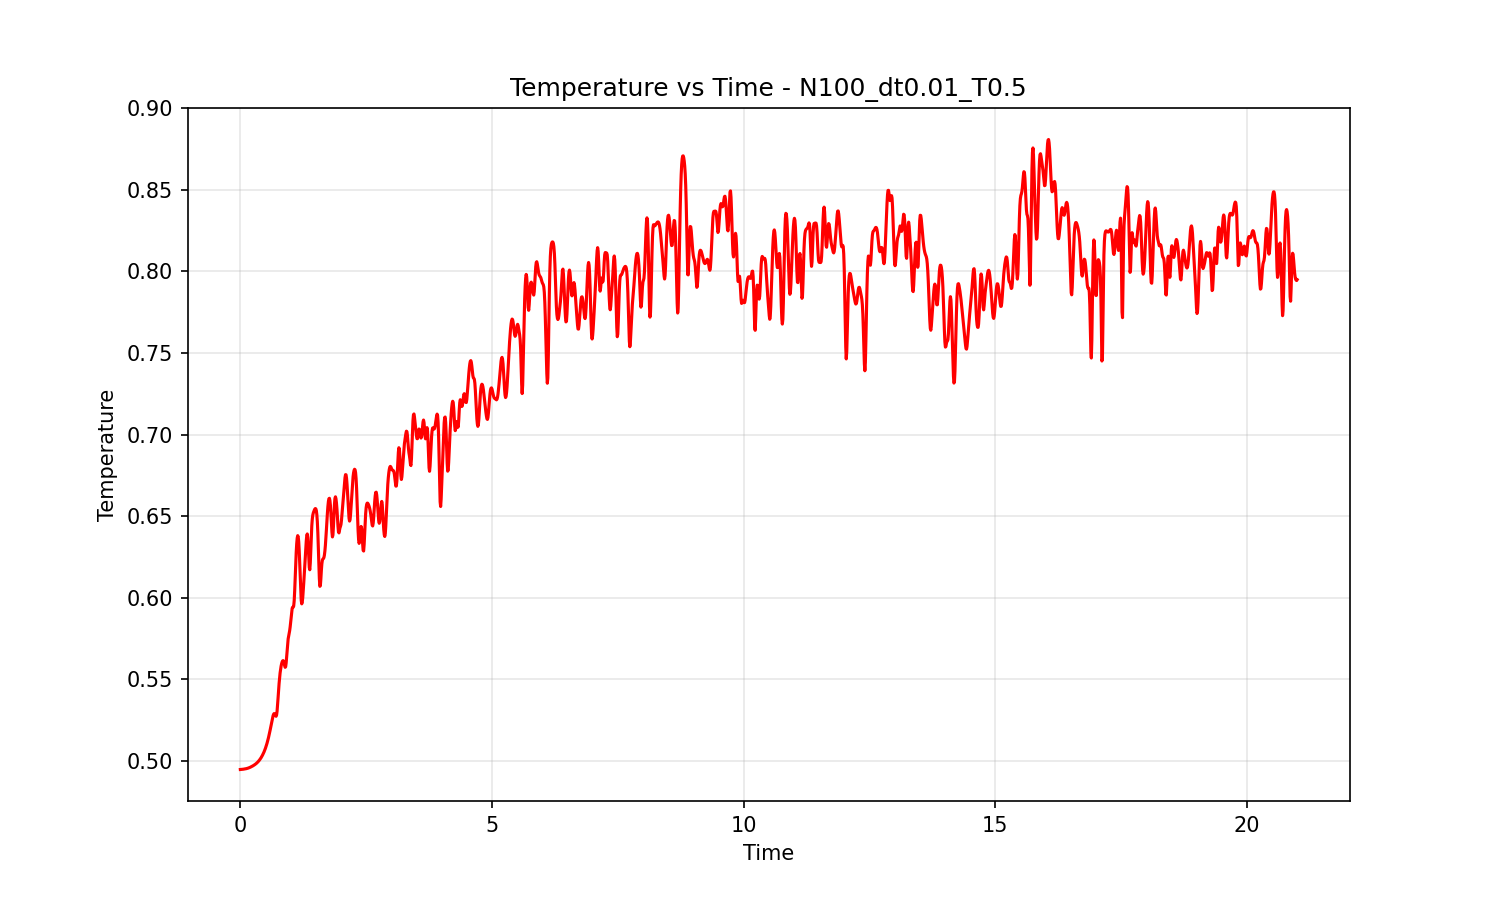
\includegraphics[width=\textwidth]{media/temp_N100_dt0.01_T0.5.png}
		\caption{N=100 particles with dt=0.01 and T=0.5}
		\label{sfig:temp_N100}
	\end{subfigure}%
	~
	\begin{subfigure}{0.5\textwidth}
		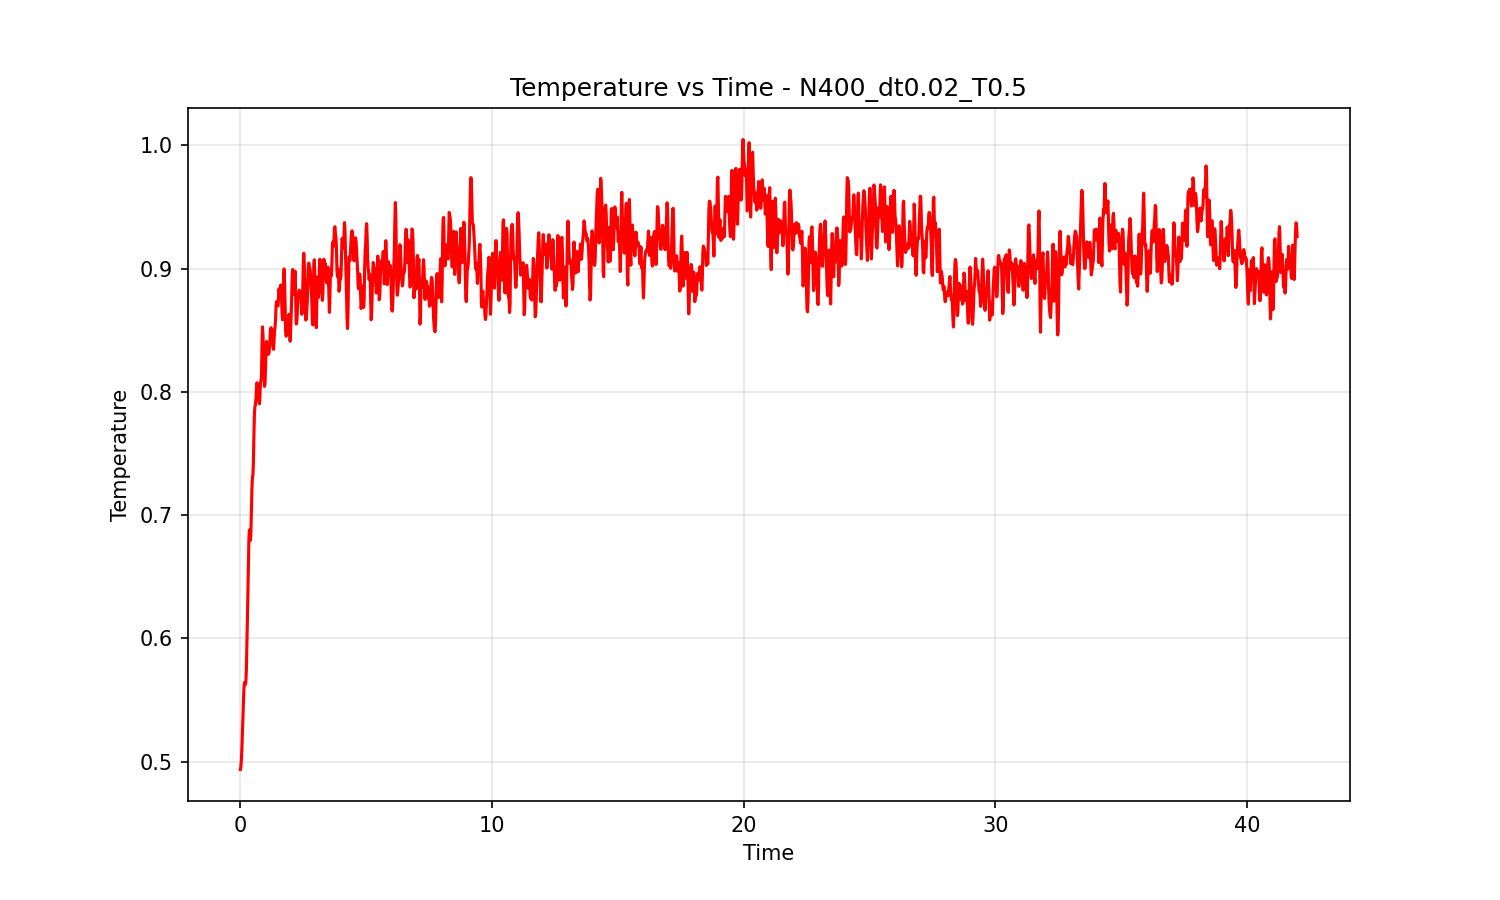
\includegraphics[width=\textwidth]{media/temp_N400_dt0.02_T0.5.png}
		\caption{N=400 particles with dt=0.02 and T=0.5}
		\label{sfig:temp_N400_dt002}
	\end{subfigure}%
	\\
	\begin{subfigure}{0.5\textwidth}
		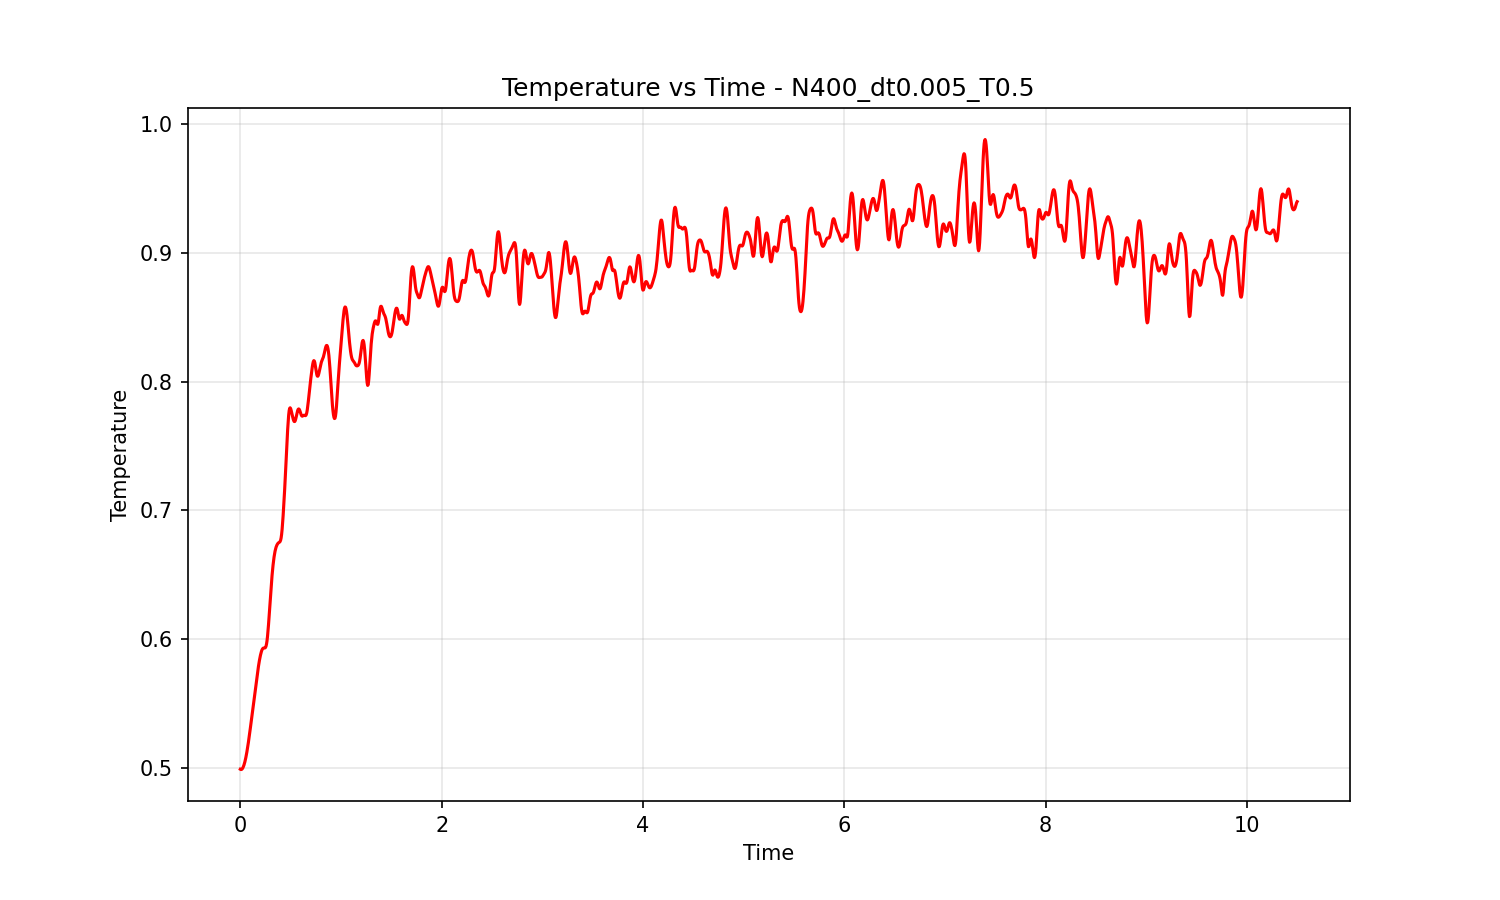
\includegraphics[width=\textwidth]{media/temp_N400_dt0.005_T0.5.png}
		\caption{N=400 particles with dt=0.005 and T=0.5}
		\label{sfig:temp_N400_dt0005}
	\end{subfigure}%
	~
	\begin{subfigure}{0.5\textwidth}
		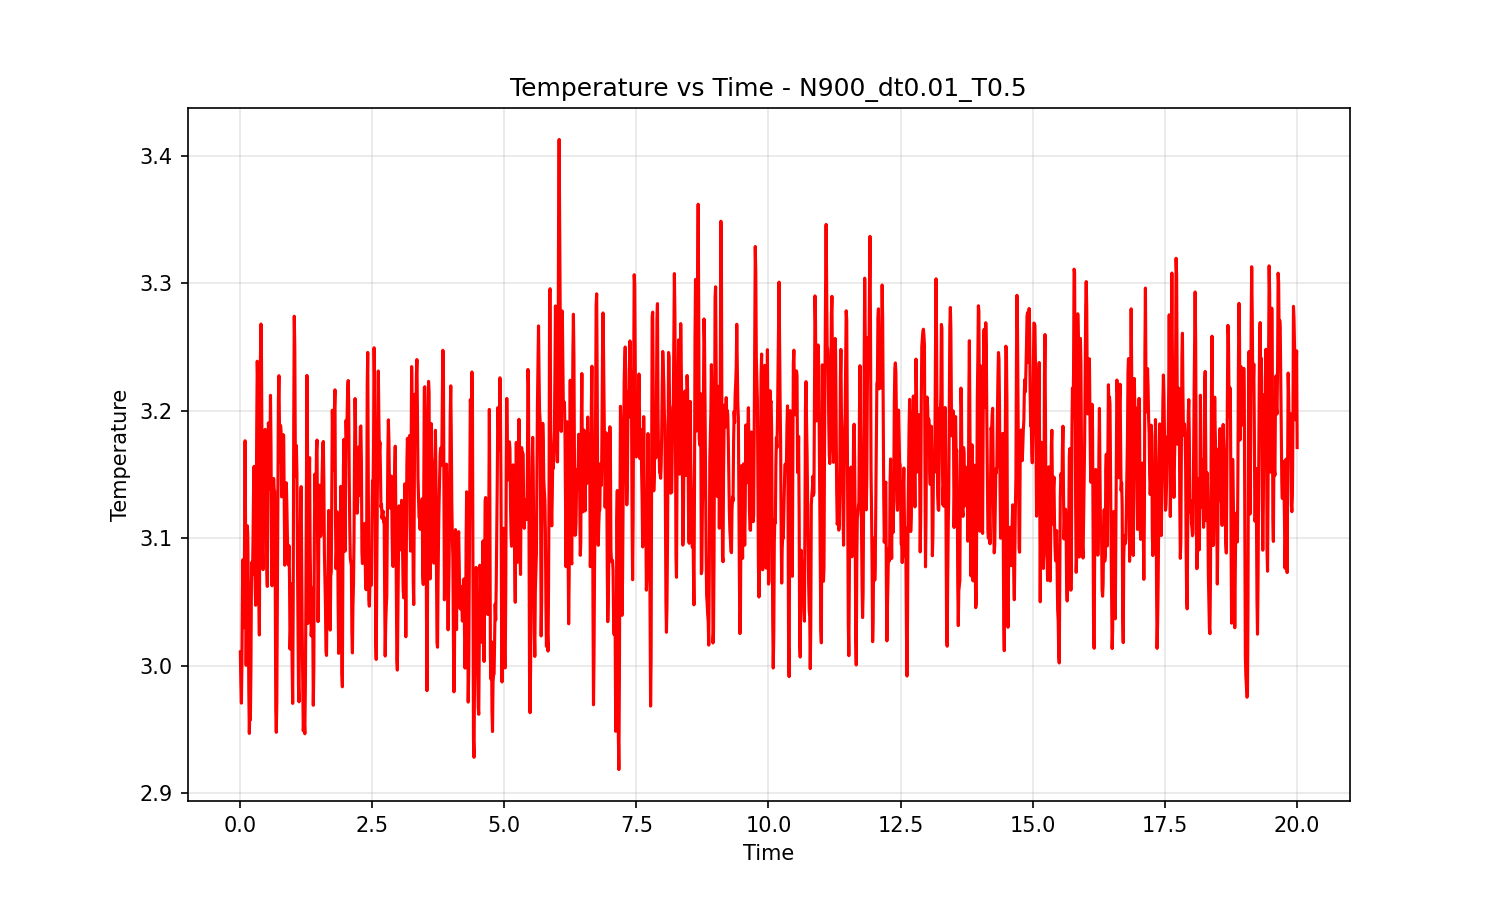
\includegraphics[width=\textwidth]{media/temp_N900_dt0.01_T0.5.png}
		\caption{N=900 particles with dt=0.01 and T=0.5}
		\label{sfig:temp_N900}
	\end{subfigure}%


	\caption{\textbf{Temperature Evolution in NVE Ensemble} 
	Analysis of temperature fluctuations over time for different system configurations.}
	\label{fig:temperature_evolution}
\end{figure}
% \begin{figure}[H]
% 	\centering
% 	\begin{subfigure}{0.5\textwidth}
% 		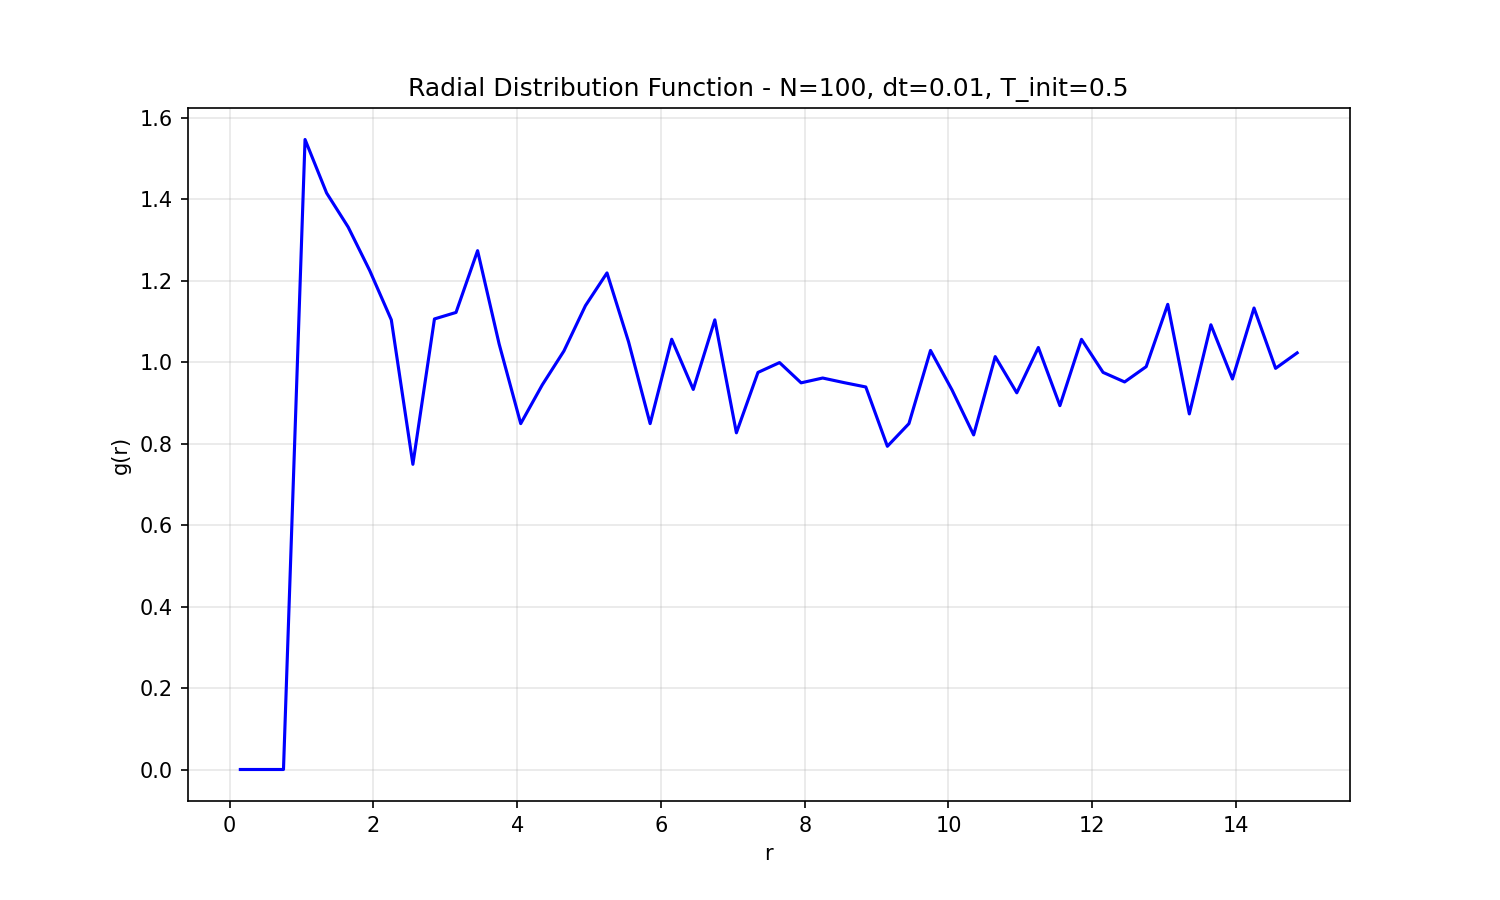
\includegraphics[width=\textwidth]{media/final_rdf_N100_dt0.01_T0.5_final.png}
% 		\caption{N=100 particles with dt=0.01 and T=0.5}
% 		\label{sfig:rdf_N100}
% 	\end{subfigure}%
% 	~
% 	\begin{subfigure}{0.5\textwidth}
% 		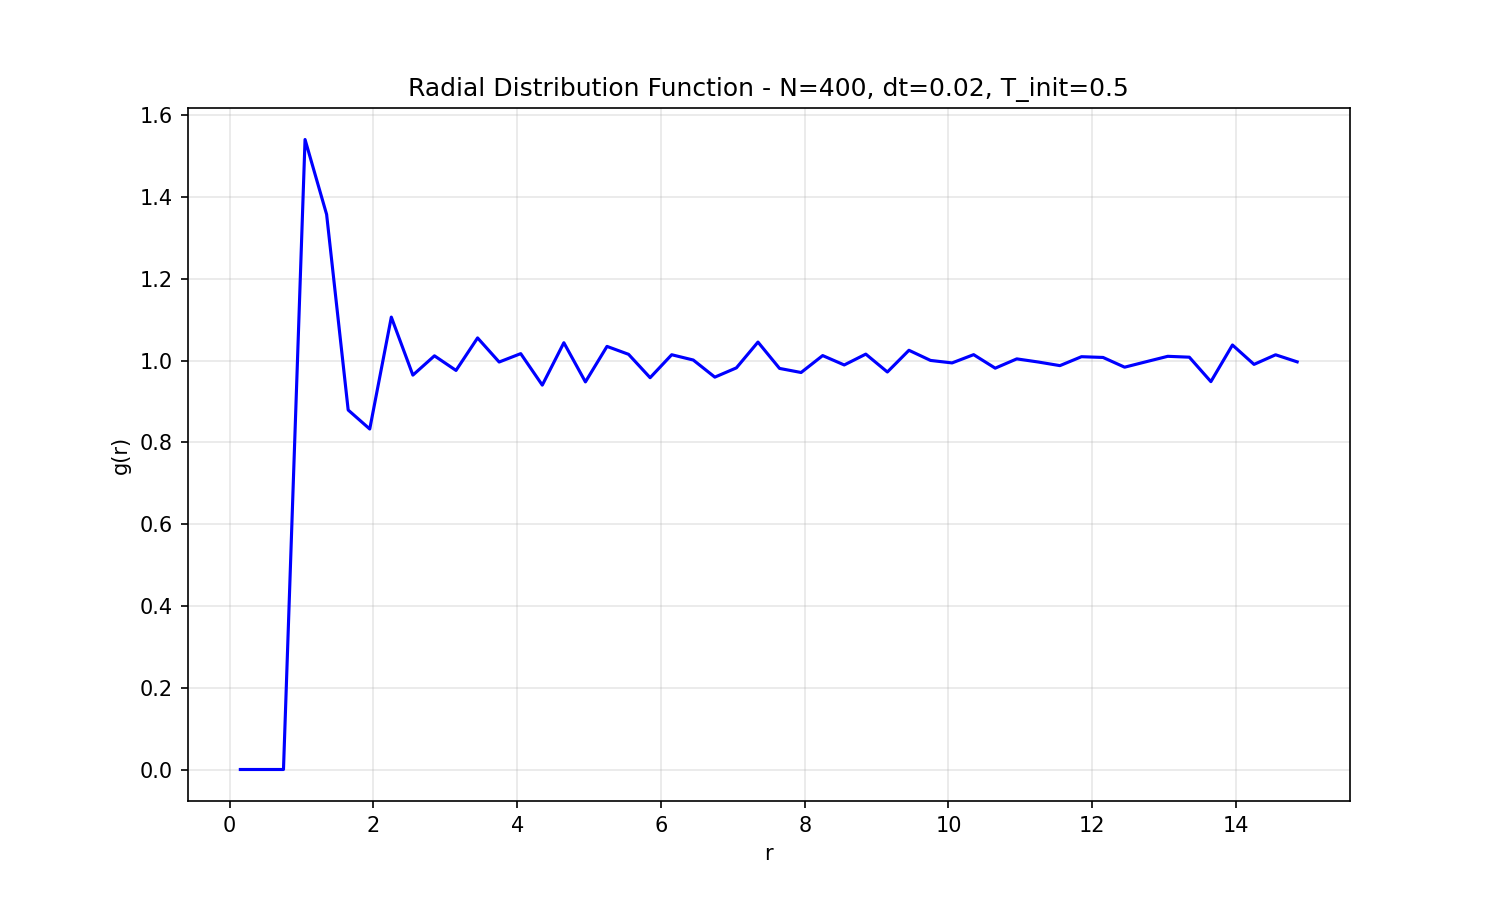
\includegraphics[width=\textwidth]{media/final_rdf_N400_dt0.02_T0.5_final.png}
% 		\caption{N=400 particles with dt=0.02 and T=0.5}
% 		\label{sfig:rdf_N400_dt002}
% 	\end{subfigure}%
% 	\\
% \begin{subfigure}{0.5\textwidth}
% 		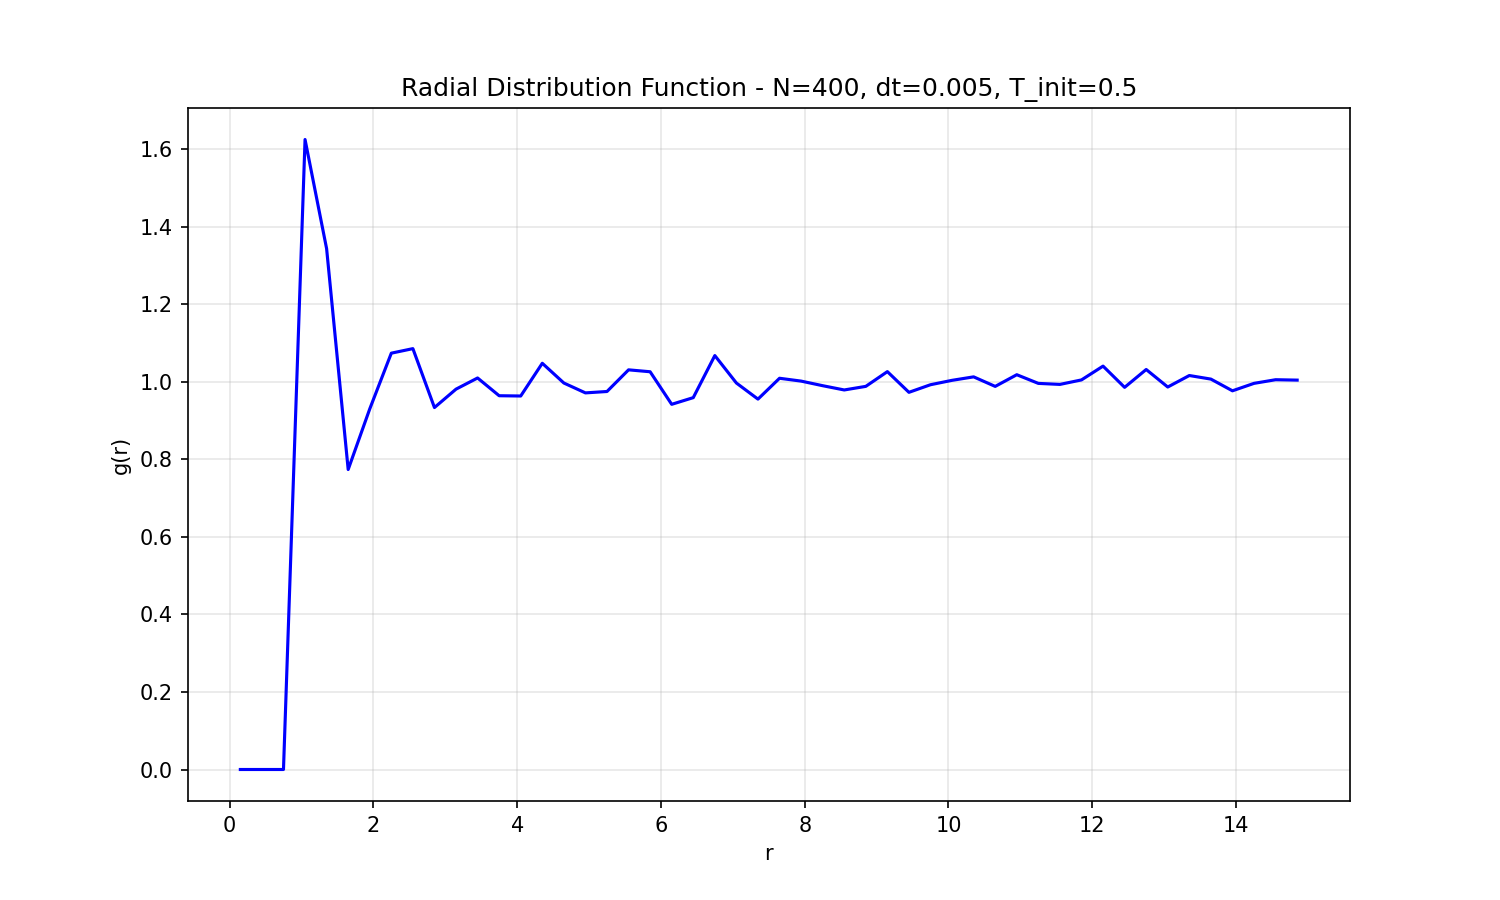
\includegraphics[width=\textwidth]{media/final_rdf_N400_dt0.005_T0.5_final.png}
% 		\caption{N=400 particles with dt=0.005 and T=0.5}
% 		\label{sfig:rdf_N400_dt0005}
% 	\end{subfigure}%
% 	~
% 	\begin{subfigure}{0.5\textwidth}
% 		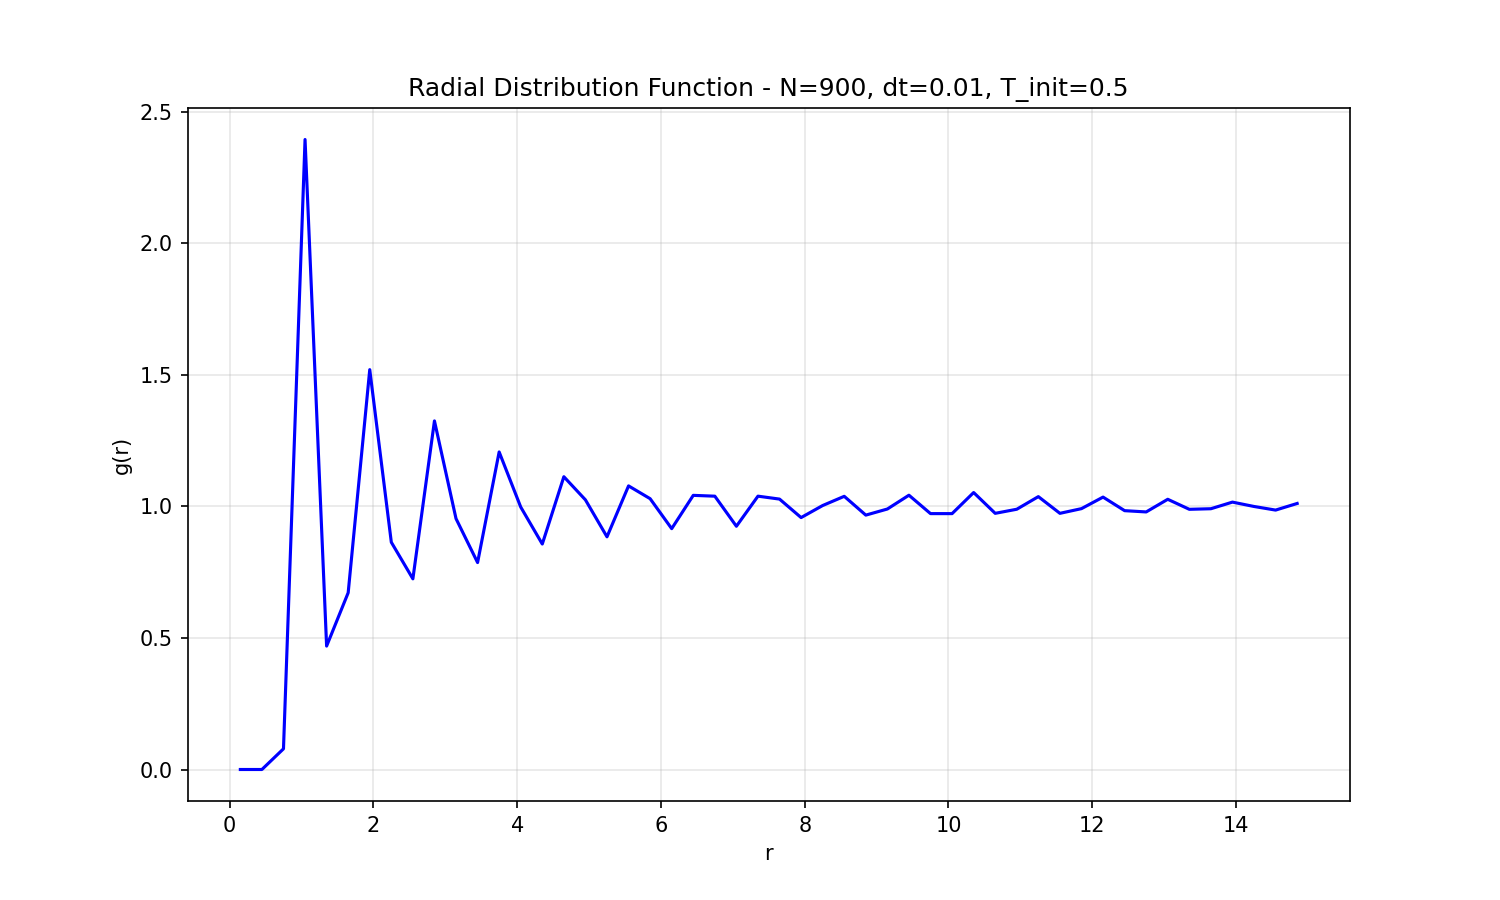
\includegraphics[width=\textwidth]{media/final_rdf_N900_dt0.01_T0.5_final.png}
% 		\caption{N=900 particles with dt=0.01 and T=0.5}
% 		\label{sfig:rdf_N900}
% 	\end{subfigure}%
% 	\caption{\textbf{Radial Distribution Functions (RDF) in NVE Ensemble} 
% 	Final radial distribution functions for different system configurations.}
% 	\label{fig:radial_distribution}
% \end{figure}
\begin{figure}[H]
	\centering
	\begin{subfigure}{0.5\textwidth}
		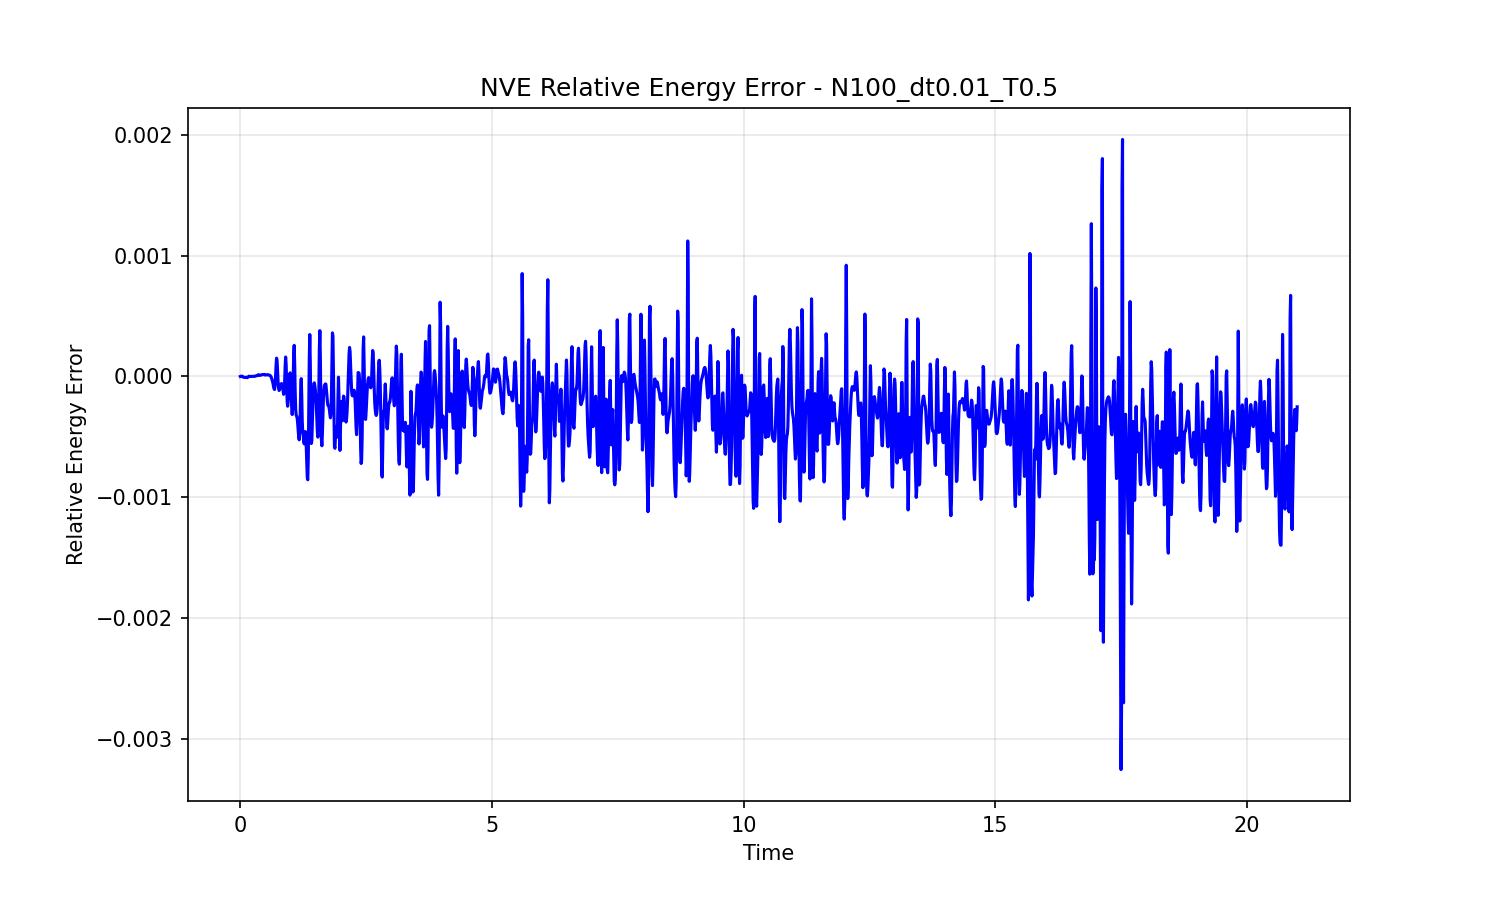
\includegraphics[width=\textwidth]{media/error_N100_dt0.01_T0.5.png}
		\caption{N=100 particles with dt=0.01 and T=0.5}
		\label{sfig:error_N100}
	\end{subfigure}%
	~
	\begin{subfigure}{0.5\textwidth}
		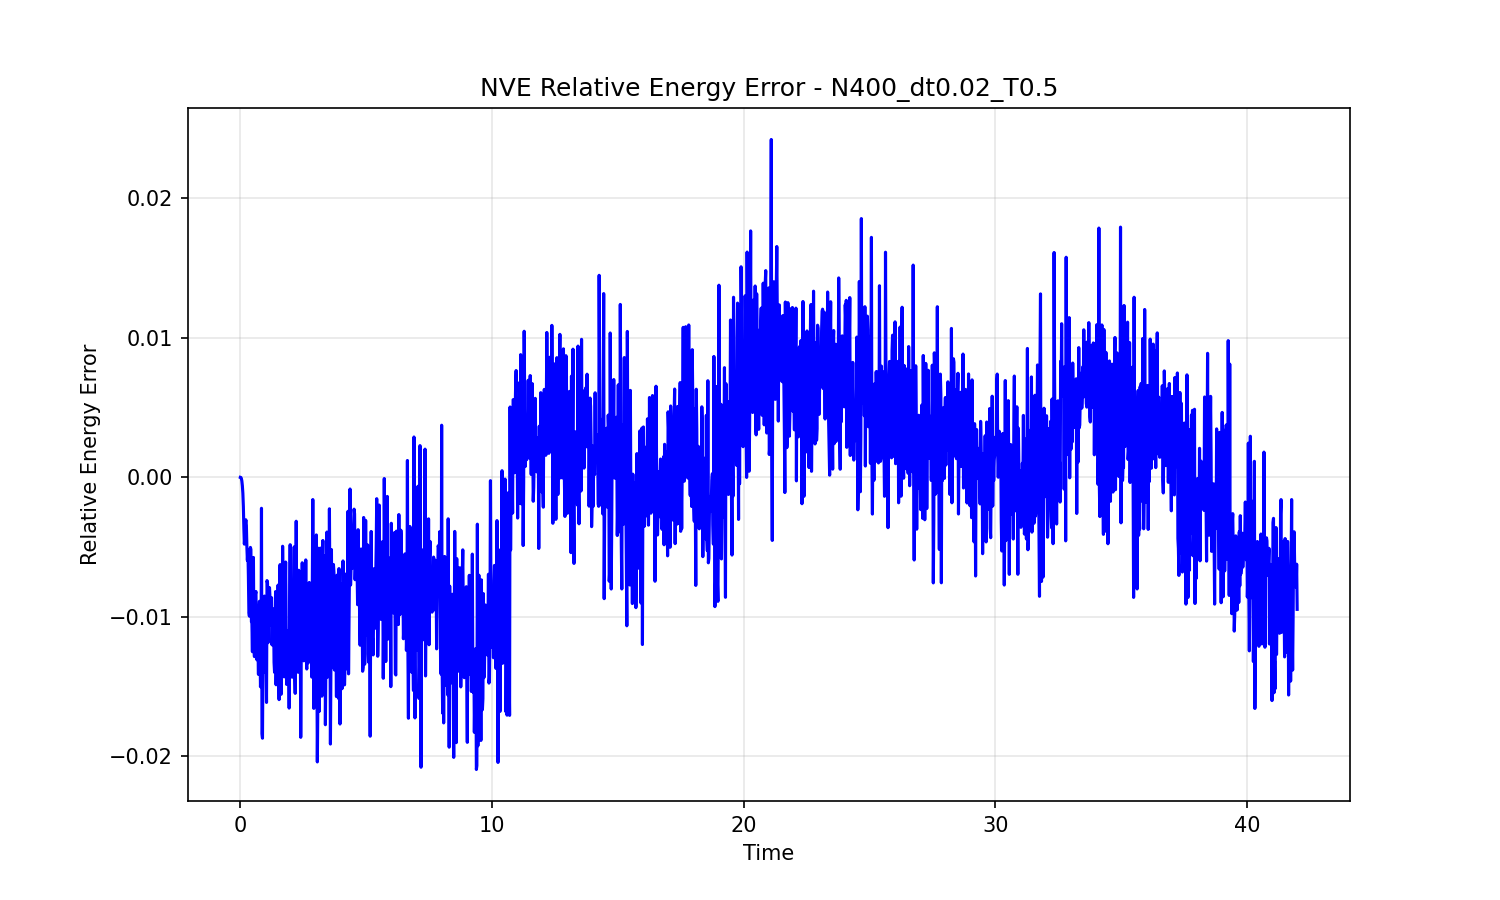
\includegraphics[width=\textwidth]{media/error_N400_dt0.02_T0.5.png}
		\caption{N=400 particles with dt=0.02 and T=0.5}
		\label{sfig:error_N400_dt002}
	\end{subfigure}%
	\\
	\begin{subfigure}{0.5\textwidth}
		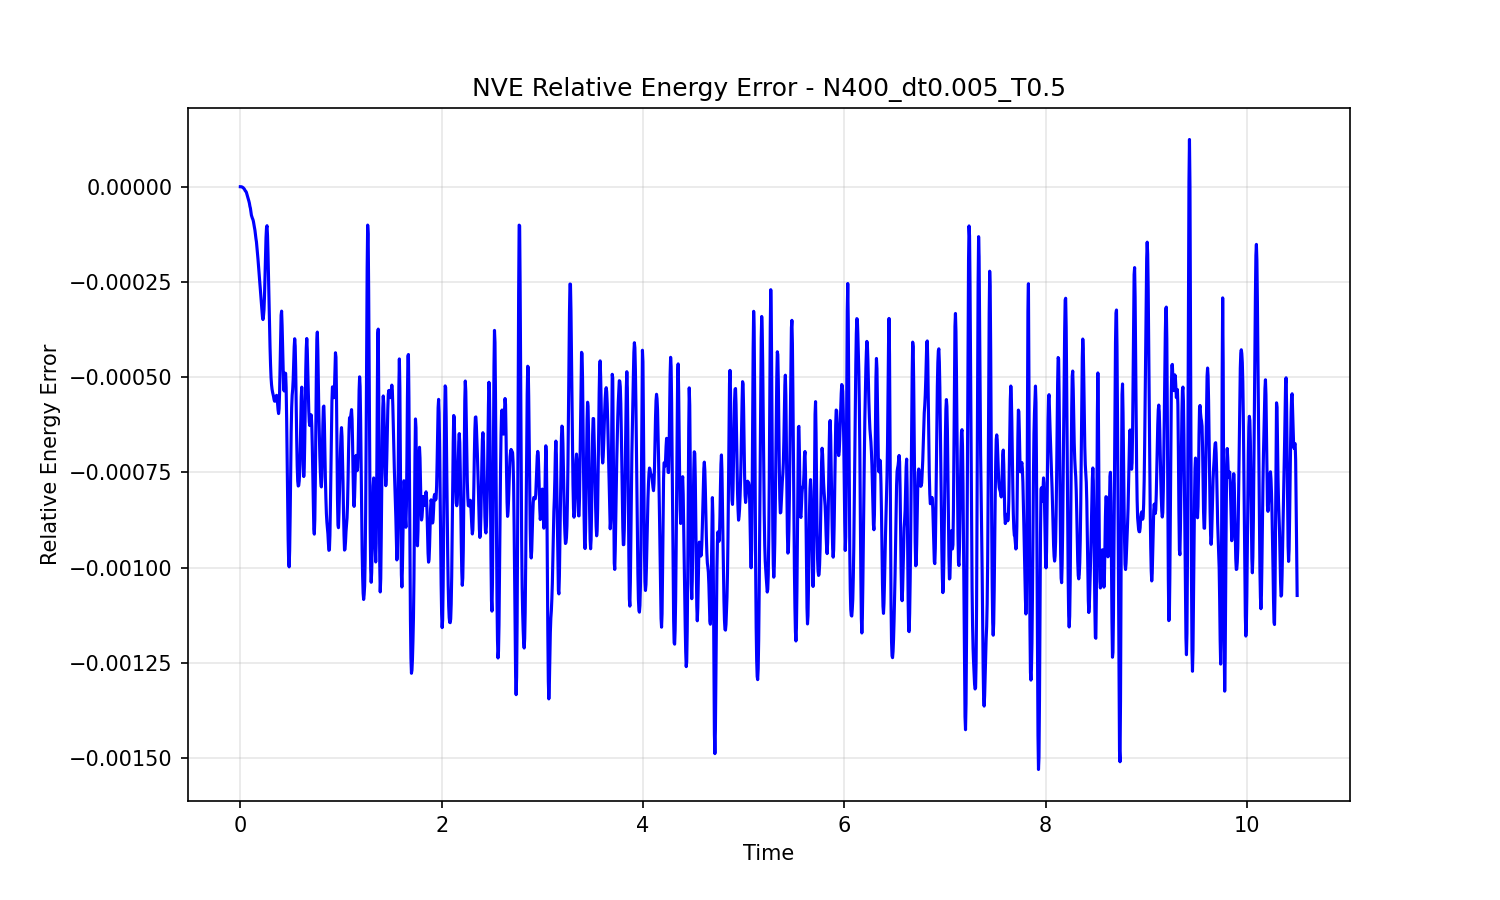
\includegraphics[width=\textwidth]{media/error_N400_dt0.005_T0.5.png}
		\caption{N=400 particles with dt=0.005 and T=0.5}
		\label{sfig:error_N400_dt0005}
	\end{subfigure}%
	~
\begin{subfigure}{0.5\textwidth}
		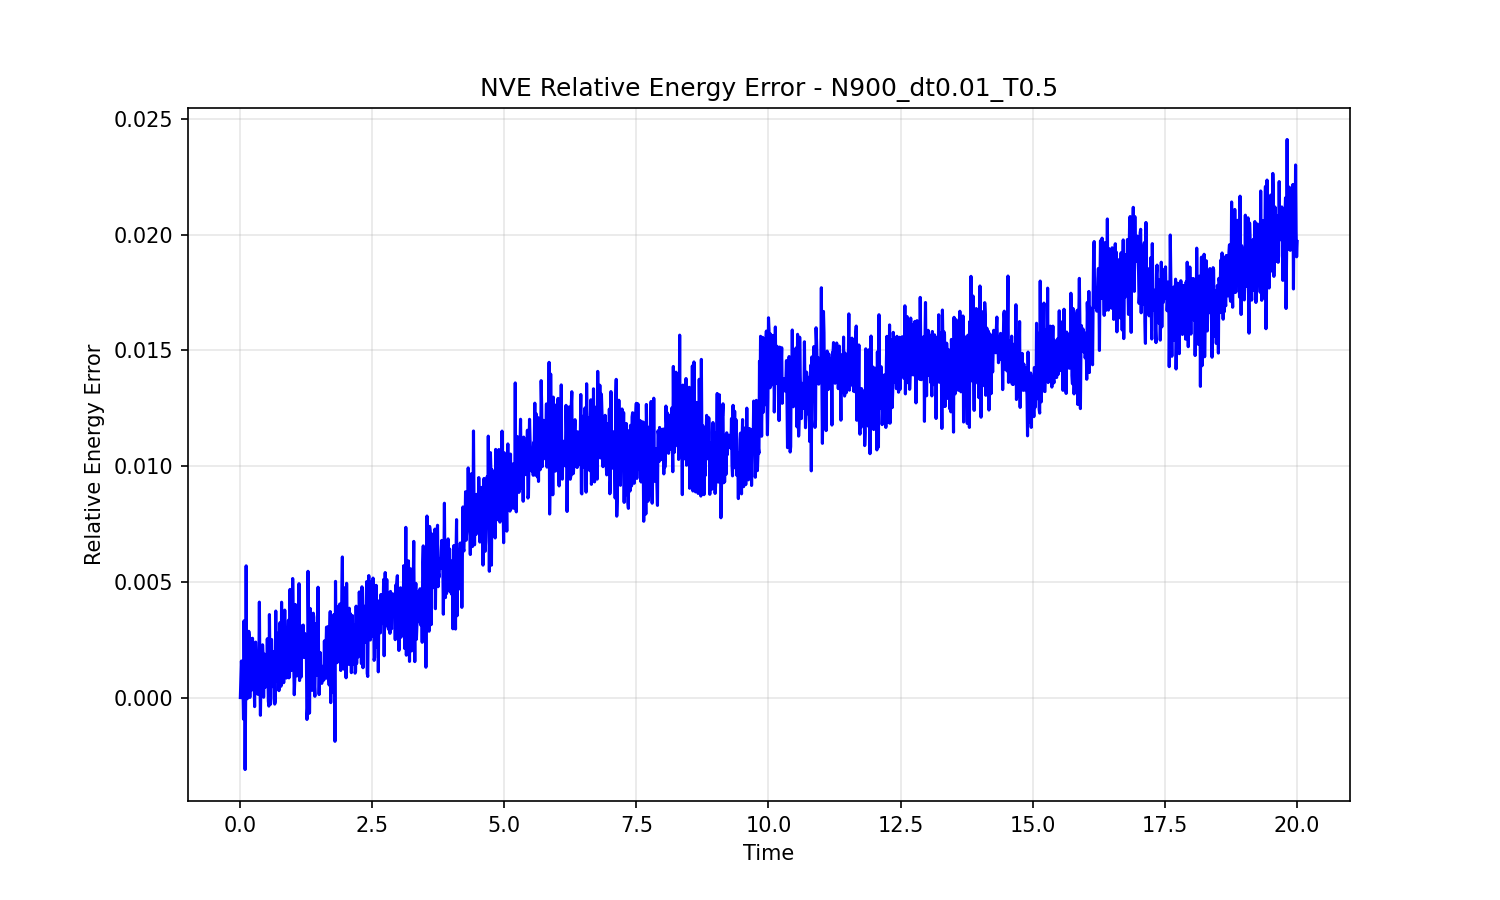
\includegraphics[width=\textwidth]{media/error_N900_dt0.01_T0.5.png}
		\caption{N=900 particles with dt=0.01 and T=0.5}
		\label{sfig:error_N900}
	\end{subfigure}%

	\caption{\textbf{Energy Conservation Error Analysis in NVE Ensemble} 
	Relative energy conservation error over time for different system configurations.}
	\label{fig:energy_error}
\end{figure}
% section Energy-Conserving Dynamics: The NVE Ensemble (end)
